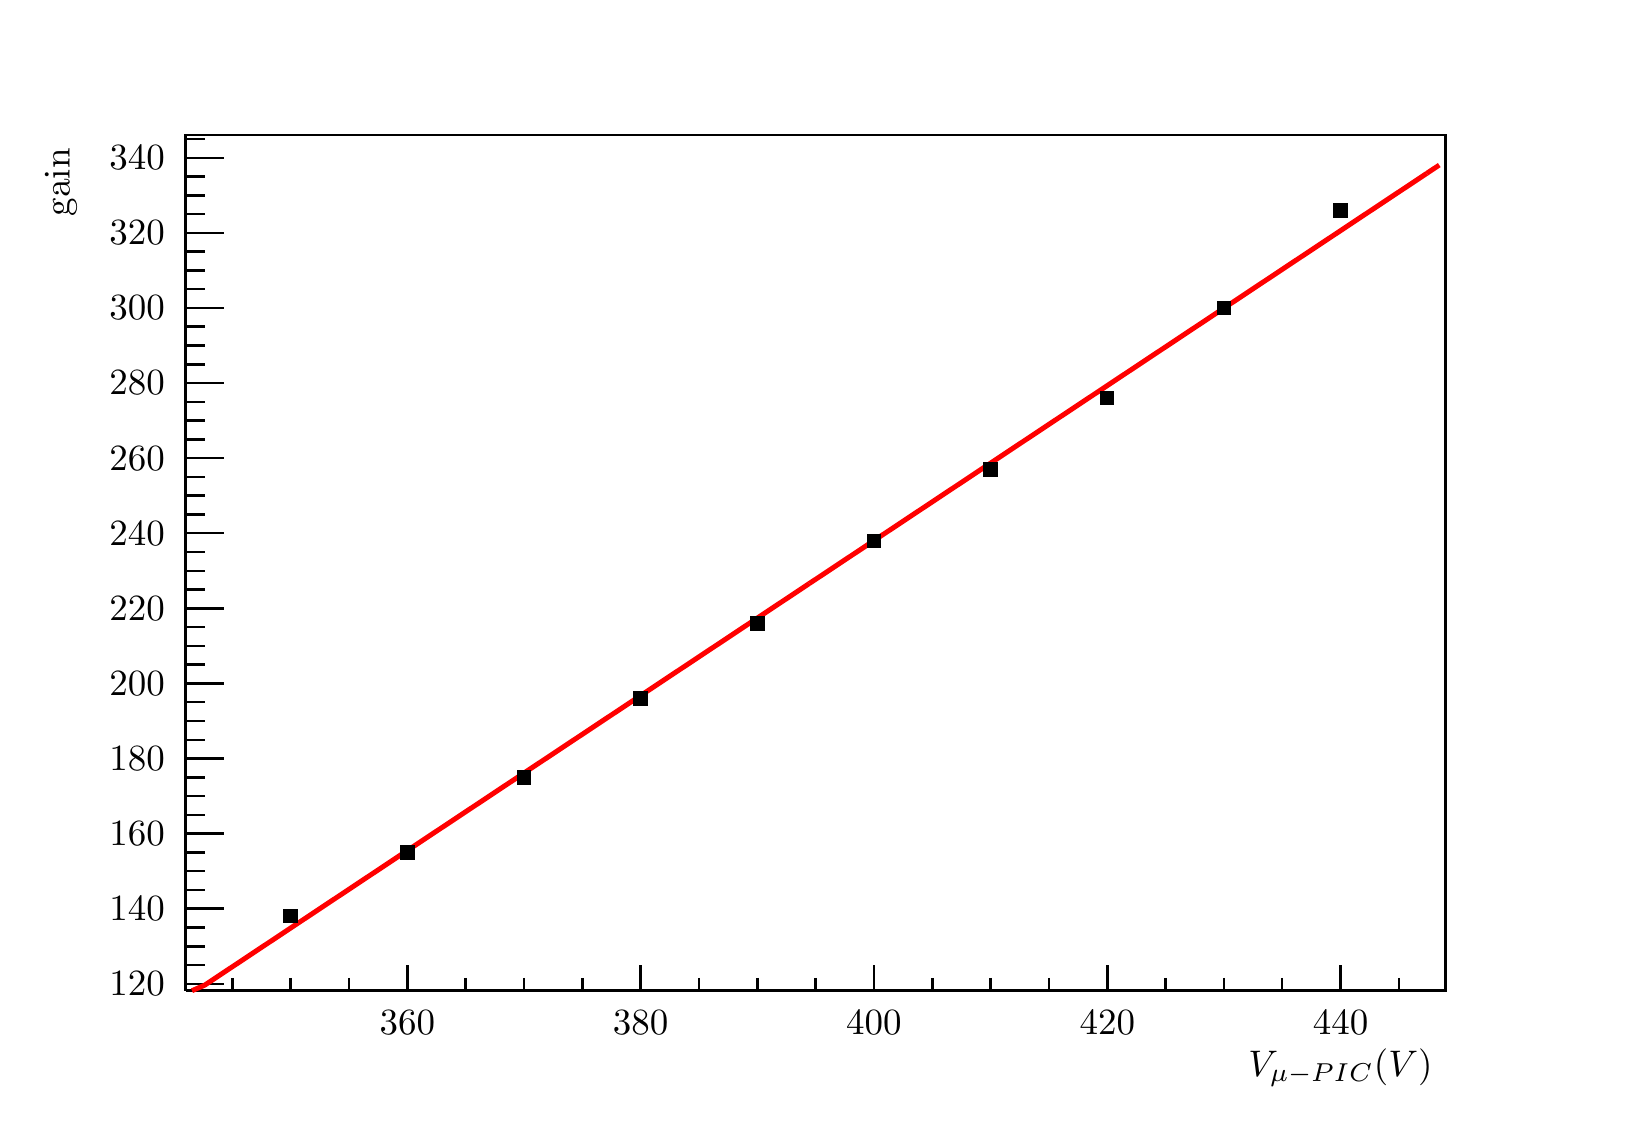
\begin{tikzpicture}
\pgfdeclareplotmark{cross} {
\pgfpathmoveto{\pgfpoint{-0.3\pgfplotmarksize}{\pgfplotmarksize}}
\pgfpathlineto{\pgfpoint{+0.3\pgfplotmarksize}{\pgfplotmarksize}}
\pgfpathlineto{\pgfpoint{+0.3\pgfplotmarksize}{0.3\pgfplotmarksize}}
\pgfpathlineto{\pgfpoint{+1\pgfplotmarksize}{0.3\pgfplotmarksize}}
\pgfpathlineto{\pgfpoint{+1\pgfplotmarksize}{-0.3\pgfplotmarksize}}
\pgfpathlineto{\pgfpoint{+0.3\pgfplotmarksize}{-0.3\pgfplotmarksize}}
\pgfpathlineto{\pgfpoint{+0.3\pgfplotmarksize}{-1.\pgfplotmarksize}}
\pgfpathlineto{\pgfpoint{-0.3\pgfplotmarksize}{-1.\pgfplotmarksize}}
\pgfpathlineto{\pgfpoint{-0.3\pgfplotmarksize}{-0.3\pgfplotmarksize}}
\pgfpathlineto{\pgfpoint{-1.\pgfplotmarksize}{-0.3\pgfplotmarksize}}
\pgfpathlineto{\pgfpoint{-1.\pgfplotmarksize}{0.3\pgfplotmarksize}}
\pgfpathlineto{\pgfpoint{-0.3\pgfplotmarksize}{0.3\pgfplotmarksize}}
\pgfpathclose
\pgfusepathqstroke
}
\pgfdeclareplotmark{cross*} {
\pgfpathmoveto{\pgfpoint{-0.3\pgfplotmarksize}{\pgfplotmarksize}}
\pgfpathlineto{\pgfpoint{+0.3\pgfplotmarksize}{\pgfplotmarksize}}
\pgfpathlineto{\pgfpoint{+0.3\pgfplotmarksize}{0.3\pgfplotmarksize}}
\pgfpathlineto{\pgfpoint{+1\pgfplotmarksize}{0.3\pgfplotmarksize}}
\pgfpathlineto{\pgfpoint{+1\pgfplotmarksize}{-0.3\pgfplotmarksize}}
\pgfpathlineto{\pgfpoint{+0.3\pgfplotmarksize}{-0.3\pgfplotmarksize}}
\pgfpathlineto{\pgfpoint{+0.3\pgfplotmarksize}{-1.\pgfplotmarksize}}
\pgfpathlineto{\pgfpoint{-0.3\pgfplotmarksize}{-1.\pgfplotmarksize}}
\pgfpathlineto{\pgfpoint{-0.3\pgfplotmarksize}{-0.3\pgfplotmarksize}}
\pgfpathlineto{\pgfpoint{-1.\pgfplotmarksize}{-0.3\pgfplotmarksize}}
\pgfpathlineto{\pgfpoint{-1.\pgfplotmarksize}{0.3\pgfplotmarksize}}
\pgfpathlineto{\pgfpoint{-0.3\pgfplotmarksize}{0.3\pgfplotmarksize}}
\pgfpathclose
\pgfusepathqfillstroke
}
\pgfdeclareplotmark{newstar} {
\pgfpathmoveto{\pgfqpoint{0pt}{\pgfplotmarksize}}
\pgfpathlineto{\pgfqpointpolar{44}{0.5\pgfplotmarksize}}
\pgfpathlineto{\pgfqpointpolar{18}{\pgfplotmarksize}}
\pgfpathlineto{\pgfqpointpolar{-20}{0.5\pgfplotmarksize}}
\pgfpathlineto{\pgfqpointpolar{-54}{\pgfplotmarksize}}
\pgfpathlineto{\pgfqpointpolar{-90}{0.5\pgfplotmarksize}}
\pgfpathlineto{\pgfqpointpolar{234}{\pgfplotmarksize}}
\pgfpathlineto{\pgfqpointpolar{198}{0.5\pgfplotmarksize}}
\pgfpathlineto{\pgfqpointpolar{162}{\pgfplotmarksize}}
\pgfpathlineto{\pgfqpointpolar{134}{0.5\pgfplotmarksize}}
\pgfpathclose
\pgfusepathqstroke
}
\pgfdeclareplotmark{newstar*} {
\pgfpathmoveto{\pgfqpoint{0pt}{\pgfplotmarksize}}
\pgfpathlineto{\pgfqpointpolar{44}{0.5\pgfplotmarksize}}
\pgfpathlineto{\pgfqpointpolar{18}{\pgfplotmarksize}}
\pgfpathlineto{\pgfqpointpolar{-20}{0.5\pgfplotmarksize}}
\pgfpathlineto{\pgfqpointpolar{-54}{\pgfplotmarksize}}
\pgfpathlineto{\pgfqpointpolar{-90}{0.5\pgfplotmarksize}}
\pgfpathlineto{\pgfqpointpolar{234}{\pgfplotmarksize}}
\pgfpathlineto{\pgfqpointpolar{198}{0.5\pgfplotmarksize}}
\pgfpathlineto{\pgfqpointpolar{162}{\pgfplotmarksize}}
\pgfpathlineto{\pgfqpointpolar{134}{0.5\pgfplotmarksize}}
\pgfpathclose
\pgfusepathqfillstroke
}
\definecolor{c}{rgb}{1,1,1};
\draw [color=c, fill=c] (0,0) rectangle (20,13.5817);
\draw [color=c, fill=c] (2,1.35817) rectangle (18,12.2235);
\definecolor{c}{rgb}{0,0,0};
\draw [c,line width=0.9] (2,1.35817) -- (2,12.2235) -- (18,12.2235) -- (18,1.35817) -- (2,1.35817);
\draw [c,line width=0.9] (2,1.35817) -- (18,1.35817);
\draw [c,line width=0.9] (4.81482,1.68413) -- (4.81482,1.35817);
\draw [c,line width=0.9] (5.55556,1.52115) -- (5.55556,1.35817);
\draw [c,line width=0.9] (6.2963,1.52115) -- (6.2963,1.35817);
\draw [c,line width=0.9] (7.03704,1.52115) -- (7.03704,1.35817);
\draw [c,line width=0.9] (7.77778,1.68413) -- (7.77778,1.35817);
\draw [c,line width=0.9] (8.51852,1.52115) -- (8.51852,1.35817);
\draw [c,line width=0.9] (9.25926,1.52115) -- (9.25926,1.35817);
\draw [c,line width=0.9] (10,1.52115) -- (10,1.35817);
\draw [c,line width=0.9] (10.7407,1.68413) -- (10.7407,1.35817);
\draw [c,line width=0.9] (11.4815,1.52115) -- (11.4815,1.35817);
\draw [c,line width=0.9] (12.2222,1.52115) -- (12.2222,1.35817);
\draw [c,line width=0.9] (12.963,1.52115) -- (12.963,1.35817);
\draw [c,line width=0.9] (13.7037,1.68413) -- (13.7037,1.35817);
\draw [c,line width=0.9] (14.4444,1.52115) -- (14.4444,1.35817);
\draw [c,line width=0.9] (15.1852,1.52115) -- (15.1852,1.35817);
\draw [c,line width=0.9] (15.9259,1.52115) -- (15.9259,1.35817);
\draw [c,line width=0.9] (16.6667,1.68413) -- (16.6667,1.35817);
\draw [c,line width=0.9] (4.81482,1.68413) -- (4.81482,1.35817);
\draw [c,line width=0.9] (4.07407,1.52115) -- (4.07407,1.35817);
\draw [c,line width=0.9] (3.33333,1.52115) -- (3.33333,1.35817);
\draw [c,line width=0.9] (2.59259,1.52115) -- (2.59259,1.35817);
\draw [c,line width=0.9] (16.6667,1.68413) -- (16.6667,1.35817);
\draw [c,line width=0.9] (17.4074,1.52115) -- (17.4074,1.35817);
\draw [anchor=base] (4.81482,0.801318) node[scale=1.3364, color=c, rotate=0]{360};
\draw [anchor=base] (7.77778,0.801318) node[scale=1.3364, color=c, rotate=0]{380};
\draw [anchor=base] (10.7407,0.801318) node[scale=1.3364, color=c, rotate=0]{400};
\draw [anchor=base] (13.7037,0.801318) node[scale=1.3364, color=c, rotate=0]{420};
\draw [anchor=base] (16.6667,0.801318) node[scale=1.3364, color=c, rotate=0]{440};
\draw [anchor= east] (18,0.380287) node[scale=1.3364, color=c, rotate=0]{$V_{\mu\text{-PIC}}\text{ (V)}$};
\draw [c,line width=0.9] (2,1.35817) -- (2,12.2235);
\draw [c,line width=0.9] (2.48,1.44571) -- (2,1.44571);
\draw [c,line width=0.9] (2.24,1.68414) -- (2,1.68414);
\draw [c,line width=0.9] (2.24,1.92256) -- (2,1.92256);
\draw [c,line width=0.9] (2.24,2.16099) -- (2,2.16099);
\draw [c,line width=0.9] (2.48,2.39942) -- (2,2.39942);
\draw [c,line width=0.9] (2.24,2.63785) -- (2,2.63785);
\draw [c,line width=0.9] (2.24,2.87627) -- (2,2.87627);
\draw [c,line width=0.9] (2.24,3.1147) -- (2,3.1147);
\draw [c,line width=0.9] (2.48,3.35313) -- (2,3.35313);
\draw [c,line width=0.9] (2.24,3.59156) -- (2,3.59156);
\draw [c,line width=0.9] (2.24,3.82999) -- (2,3.82999);
\draw [c,line width=0.9] (2.24,4.06841) -- (2,4.06841);
\draw [c,line width=0.9] (2.48,4.30684) -- (2,4.30684);
\draw [c,line width=0.9] (2.24,4.54527) -- (2,4.54527);
\draw [c,line width=0.9] (2.24,4.7837) -- (2,4.7837);
\draw [c,line width=0.9] (2.24,5.02213) -- (2,5.02213);
\draw [c,line width=0.9] (2.48,5.26055) -- (2,5.26055);
\draw [c,line width=0.9] (2.24,5.49898) -- (2,5.49898);
\draw [c,line width=0.9] (2.24,5.73741) -- (2,5.73741);
\draw [c,line width=0.9] (2.24,5.97584) -- (2,5.97584);
\draw [c,line width=0.9] (2.48,6.21426) -- (2,6.21426);
\draw [c,line width=0.9] (2.24,6.45269) -- (2,6.45269);
\draw [c,line width=0.9] (2.24,6.69112) -- (2,6.69112);
\draw [c,line width=0.9] (2.24,6.92955) -- (2,6.92955);
\draw [c,line width=0.9] (2.48,7.16798) -- (2,7.16798);
\draw [c,line width=0.9] (2.24,7.4064) -- (2,7.4064);
\draw [c,line width=0.9] (2.24,7.64483) -- (2,7.64483);
\draw [c,line width=0.9] (2.24,7.88326) -- (2,7.88326);
\draw [c,line width=0.9] (2.48,8.12169) -- (2,8.12169);
\draw [c,line width=0.9] (2.24,8.36012) -- (2,8.36012);
\draw [c,line width=0.9] (2.24,8.59854) -- (2,8.59854);
\draw [c,line width=0.9] (2.24,8.83697) -- (2,8.83697);
\draw [c,line width=0.9] (2.48,9.0754) -- (2,9.0754);
\draw [c,line width=0.9] (2.24,9.31383) -- (2,9.31383);
\draw [c,line width=0.9] (2.24,9.55225) -- (2,9.55225);
\draw [c,line width=0.9] (2.24,9.79068) -- (2,9.79068);
\draw [c,line width=0.9] (2.48,10.0291) -- (2,10.0291);
\draw [c,line width=0.9] (2.24,10.2675) -- (2,10.2675);
\draw [c,line width=0.9] (2.24,10.506) -- (2,10.506);
\draw [c,line width=0.9] (2.24,10.7444) -- (2,10.7444);
\draw [c,line width=0.9] (2.48,10.9828) -- (2,10.9828);
\draw [c,line width=0.9] (2.24,11.2212) -- (2,11.2212);
\draw [c,line width=0.9] (2.24,11.4597) -- (2,11.4597);
\draw [c,line width=0.9] (2.24,11.6981) -- (2,11.6981);
\draw [c,line width=0.9] (2.48,11.9365) -- (2,11.9365);
\draw [c,line width=0.9] (2.48,1.44571) -- (2,1.44571);
\draw [c,line width=0.9] (2.48,11.9365) -- (2,11.9365);
\draw [c,line width=0.9] (2.24,12.175) -- (2,12.175);
\draw [anchor= east] (1.9,1.44571) node[scale=1.3364, color=c, rotate=0]{120};
\draw [anchor= east] (1.9,2.39942) node[scale=1.3364, color=c, rotate=0]{140};
\draw [anchor= east] (1.9,3.35313) node[scale=1.3364, color=c, rotate=0]{160};
\draw [anchor= east] (1.9,4.30684) node[scale=1.3364, color=c, rotate=0]{180};
\draw [anchor= east] (1.9,5.26055) node[scale=1.3364, color=c, rotate=0]{200};
\draw [anchor= east] (1.9,6.21426) node[scale=1.3364, color=c, rotate=0]{220};
\draw [anchor= east] (1.9,7.16798) node[scale=1.3364, color=c, rotate=0]{240};
\draw [anchor= east] (1.9,8.12169) node[scale=1.3364, color=c, rotate=0]{260};
\draw [anchor= east] (1.9,9.0754) node[scale=1.3364, color=c, rotate=0]{280};
\draw [anchor= east] (1.9,10.0291) node[scale=1.3364, color=c, rotate=0]{300};
\draw [anchor= east] (1.9,10.9828) node[scale=1.3364, color=c, rotate=0]{320};
\draw [anchor= east] (1.9,11.9365) node[scale=1.3364, color=c, rotate=0]{340};
\draw [anchor= east] (0.416,12.2235) node[scale=1.3364, color=c, rotate=90]{gain};
\foreach \P in {(16.6667,11.2689), (15.1852,10.0291), (13.7037,8.88466), (12.2222,7.97863), (10.7407,7.07261), (9.25926,6.02352), (7.77778,5.06981), (6.2963,4.06841), (4.81482,3.1147), (3.33333,2.30405)}{\draw[mark options={color=c,fill=c},mark
 size=2.402402pt,mark=square*] plot coordinates {\P};}
\definecolor{c}{rgb}{1,0,0};
\draw [c,line width=1.8] (2.08,1.35817) -- (2.24,1.42824) -- (2.4,1.53452) -- (2.56,1.6408) -- (2.72,1.74708) -- (2.88,1.85335) -- (3.04,1.95963) -- (3.2,2.06591) -- (3.36,2.17219) -- (3.52,2.27847) -- (3.68,2.38475) -- (3.84,2.49103) -- (4,2.59731)
 -- (4.16,2.70358) -- (4.32,2.80986) -- (4.48,2.91614) -- (4.64,3.02242) -- (4.8,3.1287) -- (4.96,3.23498) -- (5.12,3.34126) -- (5.28,3.44754) -- (5.44,3.55381) -- (5.6,3.66009) -- (5.76,3.76637) -- (5.92,3.87265) -- (6.08,3.97893) -- (6.24,4.08521)
 -- (6.4,4.19149) -- (6.56,4.29776) -- (6.72,4.40404) -- (6.88,4.51032) -- (7.04,4.6166) -- (7.2,4.72288) -- (7.36,4.82916) -- (7.52,4.93544) -- (7.68,5.04172) -- (7.84,5.14799) -- (8,5.25427) -- (8.16,5.36055) -- (8.32,5.46683) -- (8.48,5.57311) --
 (8.64,5.67939) -- (8.8,5.78567) -- (8.96,5.89195) -- (9.12,5.99822) -- (9.28,6.1045) -- (9.44,6.21078) -- (9.6,6.31706) -- (9.76,6.42334) -- (9.92,6.52962);
\draw [c,line width=1.8] (9.92,6.52962) -- (10.08,6.6359) -- (10.24,6.74217) -- (10.4,6.84845) -- (10.56,6.95473) -- (10.72,7.06101) -- (10.88,7.16729) -- (11.04,7.27357) -- (11.2,7.37985) -- (11.36,7.48613) -- (11.52,7.5924) -- (11.68,7.69868) --
 (11.84,7.80496) -- (12,7.91124) -- (12.16,8.01752) -- (12.32,8.1238) -- (12.48,8.23008) -- (12.64,8.33636) -- (12.8,8.44263) -- (12.96,8.54891) -- (13.12,8.65519) -- (13.28,8.76147) -- (13.44,8.86775) -- (13.6,8.97403) -- (13.76,9.08031) --
 (13.92,9.18659) -- (14.08,9.29286) -- (14.24,9.39914) -- (14.4,9.50542) -- (14.56,9.6117) -- (14.72,9.71798) -- (14.88,9.82426) -- (15.04,9.93054) -- (15.2,10.0368) -- (15.36,10.1431) -- (15.52,10.2494) -- (15.68,10.3557) -- (15.84,10.4619) --
 (16,10.5682) -- (16.16,10.6745) -- (16.32,10.7808) -- (16.48,10.887) -- (16.64,10.9933) -- (16.8,11.0996) -- (16.96,11.2059) -- (17.12,11.3122) -- (17.28,11.4184) -- (17.44,11.5247) -- (17.6,11.631) -- (17.76,11.7373);
\draw [c,line width=1.8] (17.76,11.7373) -- (17.92,11.8436);
\definecolor{c}{rgb}{0,0,0};
\foreach \P in {(16.6667,11.2689), (15.1852,10.0291), (13.7037,8.88466), (12.2222,7.97863), (10.7407,7.07261), (9.25926,6.02352), (7.77778,5.06981), (6.2963,4.06841), (4.81482,3.1147), (3.33333,2.30405)}{\draw[mark options={color=c,fill=c},mark
 size=2.402402pt,mark=square*] plot coordinates {\P};}
\end{tikzpicture}
